%%%%%%%%%%%%%%%%%%%%%%%%%%%%%%%%%%%%%%%%%%%%%%%%%%%%%%%%%%%%%%%%%%%
%                                                                 %
%   PAW   - Reference Manual -- LaTeX Source                      %
%                                                                 %
%   Chapter 4 -- KUIP                                             %
%                                                                 %
%   EPS file      : cernlogo.eps                                  %
%                                                                 %
%   Editor: Michel Goossens / CN-AS                               %
%   Last Mod.: 15 October 1992 07:45 mg                           %
%                                                                 %
%%%%%%%%%%%%%%%%%%%%%%%%%%%%%%%%%%%%%%%%%%%%%%%%%%%%%%%%%%%%%%%%%%%

\chapter{User interface - KUIP}

\section{The PAW command structure}
\label{sec:HCOTREE}
\index{KUIP}
\index{command!structure}
\index{PAW!command structure}

All PAW commands may be seen as a path along the
PAW tree structure:

\begin{Fighere}
\epsfig{file=\EPSFIGpath/tree.eps,width=\textwidth}

\caption{Example of the PAW command tree structure}
\label{fig:TREE}
\end{Fighere}

%
%---------------------------------------------------------------------------
%
\newpage

\section{Multiple dialogue styles}
\index{multiple dialogue}
\index{dialogue style}
\index{command!mode}
\index{abbreviation}
\index{command!parameter!list}
\index{parameter!list}

PAW is based on the KUIP \cite{bib-KUIP} User Interface package,
which can provide different types of dialogue styles.
It is possible to change interactively from one style to another using
the command \PAWcind{STYLE}.
 
\subsection{Command line mode}

In command mode the user enters a command line via the terminal keyboard.

The general syntax of a \Param{command\_line}
is a \Param{command\_name} optionally followed by a \Param{parameter\_list}.
The \Param{command\_name} and \Param{parameter\_list} are
separated by one or more blanks (therefore, no blanks should appear
within the \Param{command\_name}). 
Using regular expressions notation one can write:
\begin{XMP}
command_line  ::=  command_name ( blank+ parameter_list )?
\end{XMP}
where the postfix unary operator \Lit{'+'} means ``one or more instances of the
postfixed item'' and \Lit{'?'} means ``zero or one instances of the postfixed
item''.
The parameters in the \Param{parameter\_list} are again separated by one or more
blanks:
\begin{XMP}
parameter_list  ::=  parameter ( blank+ parameter )*
\end{XMP}
where \Lit{'*'} means ``zero or more instances of the postfixed item''.
No blanks should then appear within a parameter, unless the whole parameter
is enclosed in single quotes, like for example ``This parameter has blanks''
or the blank filled parameter \Lit{' '}.

The command name is a structured name representing the path along the
inverted tree structure handled by KUIP. 
Each element of the path,
called \Param{command\_element}, is separated from the others by one slash:
\begin{XMP}
command_name  ::=  command_element ( / command_element )*
\end{XMP}

The rightmost \Param{command\_element} of a \Param{command\_name} 
must be a leaf of the tree,
i.e. a terminal \Param{command\_element}, while the others are considered menus.
The \Param{command\_name} can have up to 10 levels of command elements (i.e. 9 levels
of menus).
%
%---------------------------------------------------------------------------
%
\subsubsection{Command abbreviations}

\index{abbreviation!command}
\index{command!abbreviation}

A command can always be abbreviated, as long as it does not become
ambiguous with other commands, by omitting:

\begin{itemize}
\item the leftmost command elements
\item the rightmost characters of a command element
\end{itemize}

The shortest unambiguous abbreviation for any command is not fixed,
but depends on the whole command tree structure: KUIP takes care to list
all possible ambiguities should the user enter an ambiguous command.

The list of all executable commands can be obtained just by typing
one slash. This is a command line having a null
command element both to the left and to the right of the separator slash;
by definition a null command element is ambiguous with every non-null
command element, therefore all the available commands will be listed as
possible ambiguities.

\begin{XMPt}{Examples of ambiguous commands}
PAW > \Ucom{CONT}
*** Ambiguous command. Possible commands are :
/HISTOGRAM/2D_PLOT/CONTOUR
/HISTOGRAM/GET_VECT/CONTENTS
/HISTOGRAM/PUT_VECT/CONTENTS
PAW > \Ucom{PUT_VECT/CONTENTS}
Histogram Identifier (<CR>=110): \Ucom{100}
Vector name (<CR>=XYZ): \Ucom{VEC}

PAW > \Ucom{P/C}
*** Ambiguous command. Possible commands are :
/HISTOGRAM/PUT_VECT/CONTENTS
/PICTURE/CREATE
/PICTURE/COPY
 
PAW > \Ucom{P/CO}
*** Ambiguous command. Possible commands are :
/HISTOGRAM/PUT_VECT/CONTENTS
/PICTURE/COPY
PAW > \Ucom{PU/C}
Histogram Identifier (<CR>=100): \Ucom{110}
Vector name (<CR>=VEC): \Ucom{VV}
\end{XMPt}

The shortest unambiguous abbreviation for any command is not fixed,
but depending on the whole command tree structure: KUIP takes care to list
all possible ambiguities should the user have entered an ambiguous command.
 
The list of all executable commands can be obtained just by typing
one slash. This is a command line having a null
command element both to the left and to the right of the separator slash;
by definition a null command element is ambiguous with every non-null
command element, therefore all the available commands will be listed as
possible ambiguities.

%
%---------------------------------------------------------------------------
%
\subsubsection{Parameters}

\index{parameter}
\index{command!parameter}

As explained above, a command line consists of a {\bf command} part optionally
followed by a {\bf parameter} part.
For example, the PAW command \Command{\tt NTUPLE/LIST}
has no parameters, while \Command{NTUPLE/PRINT} has one parameter,
i.e. the Ntuple identifier. 

\begin{XMPt}{Using the {\tt USAGE} command}
PAW > \Ucom{USAGE NTUPLE/LIST}

 * NTUPLE/LIST

PAW > \Ucom{USAGE NTUPLE/PRINT}

 * NTUPLE/PRINT  IDN
\end{XMPt}

Parameters can be {\bf mandatory} or {\bf optional}. 
For example the command \Command{ZEBRA/DZ/STORE}
has one optional parameter, i.e. the ``ZEBRA store number''.
An optional parameter always has a {\bf default value},
\index{default value}
which is used when the user does not specify the parameter. 
In the example above the default value is \Lit{0},
therefore entering just \PAWcind{STORE} is equivalent to \Command{STORE 0}.

\newpage

On the other hand the command \Command{ZEBRA/FZ/TOALPHA}
has one mandatory parameter, i.e. the name of a FZ text file.
If the user enters just \Command{TOALPHA}, 
he will be prompted also for the file name:
\begin{XMP}
PAW > \Ucom{TOALPHA}
Name of the FZ text file (<CR>=FF.DAT): \Ucom{GG.DAT}
\end{XMP}

The {\bf order}
\index{order}
of parameters in the command line is important and must match
the semantic definition of the command.
Mandatory parameters are always specified before any
optional parameters.

An {\bf exclamation mark}
\index{exclamation mark}
may be used as default value filler character.
As an example consider the following PAW command:
\begin{XMP}
PAW > \Ucom{USAGE NTUPLE/PLOT}
 * NTUPLE/PLOT  IDN [ UWFUNC NEVENT IFIRST NUPD CHOPT ]
\end{XMP}
which has one mandatory and five optional parameters.
If only the fourth parameter, \Param{IFIRST}, needs to be specified
(hence taking the default
values for all other optional parameters), then one may enter:
\begin{XMP}
PAW > \Ucom{NTUPLE/PLOT 30 ! ! 1000}
\end{XMP}

Parameters can be entered in command lines also by their name, i.e.
independently from their position. This is particularly useful when
an optional parameter has to be specified for a command with several
optional parameters. 
Values are assigned to parameters by indicating
the name of the parameter, followed by an equal sign, followed by the
value, with no blanks in between 
(see first line of the example below).
When the parameter's name is \Param{CHOPT} a shortcut is possible:
a minus sign preceding a (non-numerical) value means \Command{'CHOPT='}
(see third and fourth line of the example below).
If a parameter (with no \Command{NAME=}) is specified after a named
parameter, it will refer to the parameter following the named one
(see second line of the example below).

For example, consider the following command:
\begin{XMP}
 NTUPLE/PLOT  IDN [ UWFUNC NEVENT IFIRST NUPD CHOPT ]
\end{XMP}

One could then enter:

\begin{tabular}{>{\tt}l@{\quad}l}
 \Ucom{N/PL 123.x NUPD=100}   & instead of \Ucom{N/PL 123.x ! ! ! 100} \\
 \Ucom{N/PL NEVENT=1000 500}  & instead of \Ucom{N/PL idn ! 1000 500}  
                                     (\Rarg{idn} must be given interactively)  \\
 \Ucom{N/PL 123.x CHOPT=B}    & instead of \Ucom{N/PL 123.x ! ! ! ! B} \\
 \Ucom{N/PL 123.x -B}         & same as above
\end{tabular}

\index{parameter names}
\index{abbreviation}
Note that, unlike command elements, parameter names cannot be abbreviated.
%
%---------------------------------------------------------------------------
%
\newpage
\subsection{An overview of KUIP menu modes}

Only a short overview is given here. See the KUIP manual for more details.

\index{alphanumeric!menu mode}
\index{graphical!menu mode}
\index{menu!mode}
\index{KUIP!STYLE}
\index{STYLE!AN}
\index{STYLE!G}
\index{STYLE!GP}
\index{panel}
\index{pull-down menu}
\index{menu!alphanumeric}
\index{menu!graphical!pull-down}
\index{menu!graphical!panel}
\index{command!{\tt STYLE AN}}
\index{command!{\tt STYLE AL}}
\index{alphanumeric mode}

{\bf Alphanumeric}, entered by \Command{STYLE AN} or \Command{STYLE AL}.

The desired command is selected from a list by number or by letter.

{\bf Graphics}, entered by \Command{STYLE G} or \Command{STYLE GP}.
\index{graphics mode}
This mode is particularly interesting for workstations.
It should not be used with simple terminals.
 
\begin{minipage}{.49\textwidth}
\begin{itemize}
\item \Command{STYLE G}: Pull-down menus,
\index{command!STYLE G}
fixed layout, reflecting the command structure;
\end{itemize}
\end{minipage} \hfill
\begin{minipage}{.49\textwidth}
\begin{Fighere}
\begin{center}
\mbox{\epsfysize.2\textheight\epsfbox{styleg.eps}}
\end{center}
\end{Fighere}
\end{minipage} 

\begin{minipage}[t]{.49\textwidth}
\begin{itemize}
\item \Command{STYLE GP}: Panels of function keys, allowing
\index{command!STYLE GP}
interactive user definable multiple layouts.
\end{itemize}
\end{minipage} \hfill
\begin{minipage}{.49\textwidth}
\begin{Fighere}
\begin{center}
\mbox{\epsfysize.2\textheight\epsfbox{stylegp.eps}}
\end{center}
\end{Fighere}
\end{minipage} 

\begin{minipage}[t]{.49\textwidth}
{\bf Motif}
\index{MOTIF}
\index{OSF}
\index{command!STYLE M}
This mode, to be released soon, is suited for X11 based WorkStations
or X-terminals.
\end{minipage} \hfill
\begin{minipage}{.49\textwidth}
\begin{Fighere}
\begin{center}
\mbox{\epsfysize.23\textheight\epsfbox{stylem.eps}}
\end{center}
\end{Fighere}
\end{minipage} 

{\bf User}:
\index{user mode}
\index{command!{\tt STYLE U}}

This mode must be used in conjunction with routine \Rind{KUSER}
(see KUIP manual).
 
%
%---------------------------------------------------------------------------
%
\newpage
\section{Macros}

\index{macro}
\index{exec}
\index{macro!statements}
\index{macro!READ}
\index{macro!RETURN}
\index{macro!ON ERROR GOTO}
\index{macro!GOTO}
\index{macro!IF}
\index{READ macro statement}
\index{RETURN macro statement}
\index{ON ERROR GOTO macro statement}
\index{GOTO macro!statement}
\index{IF macro!statement}
\index{label!in KUIP macro}
\index{macro!label}

A macro is a set of command lines stored in a file,
which can be created/edited with a local editor
and executed with the command \Command{EXEC}. For example the command

\begin{XMP}
PAW > \Ucom{EXEC MNAME}
\end{XMP}

executes the command lines contained in the macro file \Lit{MNAME}.
As a macro file can contain several macros, a dash sign (\Lit{\#})
is used to select a particular macro inside a file:

\begin{itemize}
\item If \Lit{MNAME} does not contain the character '\Lit{#}', the file
      \Lit{MNAME.KUMAC}
      is searched and the first macro is executed (it may be an unnamed
      macro if a \Lit{MACRO} statement is not found as first command
      line in the file)
\item If \Lit{MNAME} is of the form \Lit{FILE#MACRO},
      the file named \Lit{FILE.KUMAC} is searched and the macro named
      \Lit{MACRO} is executed
\end{itemize}
 
\begin{XMPt}{Example of macro calls}
PAW > \Ucom{EXEC ABC}   | Execute first (or unnamed) macro of file ABC.KUMAC
PAW > \Ucom{EXEC ABC#M} | Execute macro M of file ABC.KUMAC
\end{XMPt}

In addition to all available KUIP commands the 
special ``macro statements'' in table \ref{Tab:Macrocom}
\index{macro!statements} 
are valid only inside macros (except for \PAWcind{EXEC}, which is valid 
both inside and outside)
In the last line of the table \Lit{par} stands for either 
an argument passed with the command \Command{EXEC}
(in the command mode or from another macro)
or a local variable of the macro.

\Lit{arithmetic\_expression} and
\Lit{logical\_expression} are expressions with only two terms,
which are defined as follows (``\Lit{|}'' stands for ``or'' 
and juxtaposition stands for ``and''):
\index{operand}
\index{arithmetic!expression}
\index{arithmetic!operator}
\index{logical!expression}
\index{logical!operator}
\begin{XMP}
operand                 =   par  |  constant
arithmetic_expression   =   operand  arithmetic_operator  operand
arithmetic_operator     =   +  |  -  |  *  |  /
logical_expression      =   operand  logical_operator  operand
logical_operator        =   =  |  <  |  <=  |  >  |  >=  |  <>
\end{XMP}

A label is any string in a line that is terminated by a colon
(therefore labels must stand alone on a line).
A label definition is local to a macro, so that
the same label can be re-used in different macros.

The \Lit{ON ERROR GOTO} 
\index{ON ERROR GOTO}
statement is activated by error conditions of the
system and by the application program%
\footnote{More precisely,
after execution of a line inside a macro, the variable
\PAWcind[QUEST]{IQUEST(1)} (in \Lit{COMMON/QUEST/IQUEST(100)}) is checked. 
If it is different from \Lit{0}, then the \PAWcind{ON ERROR GOTO} logic is triggered.}.
In executing a macro, the latest \Command{ON ERROR GOTO} executed is the active one
(i.e. the previous one is superseded).

\newpage
\begin{Tabhere}
\begin{center}
\begin{tabular}{|>{\tt}l|l|} \hline
\multicolumn{2}{|c|}{\bf Macro Statements} \\ \hline 
{\sc Statement}                       & {\sc Description}                                         \\ 
\hline
\PAWcind{MACRO} mname par1=val1 ...             & begin macro \Lit{mname}                                   \\ 
\PAWcind{EXEC} mname par1 par2=val2 ...         & execute macro \Lit{mname}                                 \\ 
\PAWcind{RETURN}                                & end of a macro                                            \\ 
\PAWcind{READ} par                              & read macro parameter \Lit{par} from keyboard              \\ 
\PAWcind{SHIFT}                                 & control parameters list                                   \\ 
\PAWcind{label:}                                & label (must terminate with a colon)                       \\ 
\PAWcind{GOTO} label                            & jump to \Lit{label}                                       \\ 
\PAWcind{ON ERROR GOTO} label                   & resume at \Lit{label} on error condition                  \\ 
\PAWcind{OF ERROR}                              & temporarily deactivate the \Lit{ON ERROR GOTO} handling   \\ 
\PAWcind{ON ERROR}                              & reactivate the latest \Lit{ON ERROR GOTO} handling        \\ 
\PAWcind{IF} logical\_expression GOTO label     & conditional statement                                     \\ 
IF-THEN, ELSEIF, \PAWcind{ELSE}, ENDIF          & Macro flow control                                        \\ 
\PAWcind{CASE}, ENDCASE                         & Macro flow control                                        \\ 
\PAWcind{WHILE}-DO, ENDWHILE                    & Macro flow control                                        \\ 
\PAWcind{REPEAT}, \PAWcind{UNTIL}               & Macro flow control                                        \\ 
\PAWcind{DO}, ENDDO                             & Macro flow control                                        \\ 
\PAWcind{FOR}, ENDFOR                           & Macro flow control                                        \\ 
\PAWcind{BREAKL}                                & Macro flow control                                        \\ 
\PAWcind{EXITM}                                 & Macro termination                                         \\ 
par = arithmetic\_expression                    & assignment statement                                      \\ 
\hline
\end{tabular}
\end{center}
\caption{List of statements possible inside KUIP macros}
\index{macro!statements}
\label{Tab:Macrocom}
\end{Tabhere}

Positional parameters can be passed to a macro, separated by blanks.
Inside a macro, positional parameters can be retrieved by including
in brackets the number representing their order in the list.
\index{parameters}
\index{macro}

\begin{XMPin}{Example of macro file}
MACRO ABC
  MESSAGE [1] [3] [2]
RETURN
\end{XMPin}
\begin{XMPout}{Example of macro execution}
PAW > \Ucom{EXEC ABC P1 123 'This is P3'}

P1 This is P3 123
\end{XMPout}

Note that normal variables are not translated if they have not been assigned a
value, whereas unassigned positional parameters are {\bf always} replaced by the
blank character \Lit{' '}.
Macro parameters can be concatenated to anything in the command line;
whenever a parameter number (or name - see below), enclosed in brackets,
is encountered in the command line, it will be substituted by its
value before execution of the command line. 

\begin{XMPin}{Example of macro file}
MACRO OPEN
  HISTO/FILE 20 DST[1].DAT
RETURN
\end{XMPin}
\begin{XMPout}{Example of parameter substitution}
PAW > \Ucom{EXEC OPEN 123TEST}
{\rm will execute the command:}
HISTO/FILE 20 DST123TEST.DAT
\end{XMPout}

Non-positional (i.e. named) parameters can also be passed.
This is useful when several parameters are associated to a macro.
Initial values of parameters should be specified in the \Command{MACRO} statement.
For example, changing the macro \Lit{OPEN} above to:

\begin{XMPt}{Example of macro with lot of parameters}
MACRO OPEN LUN=20 NAME=JUNK EXT=DAT LRECL=1024 CHOPT=' '
  HISTO/FILE [LUN] [NAME].[EXT] [LRECL] [CHOPT]
RETURN
\end{XMPt}

\begin{XMPin}{Example of macro call}
PAW > \Ucom{EXEC OPEN EXT=TEMP LUN=10}
\end{XMPin}
\begin{XMPout}{Output generated by macro call}
HISTO/FILE 10 JUNK.TEMP 1024
\end{XMPout}

Parameters can also be read in at macro run time. 
When a \PAWcind{READ} statement is executed
the user will be asked to provide values for the given parameters.
If just \Lit{<CR>} is entered, the values remain unchanged.
\begin{XMPt}{Example of macro reading parameters at run time}
MACRO INP
  READ PPP
  READ 1
  MESSAGE 'The value of the parameter PPP is ... ' [PPP]
  MESSAGE 'The value of the parameter 1 is ..... ' [1]
RETURN
\end{XMPt}
The order of priority for macro parameters is such that the values given
in the \PAWcind{EXEC} statement supersede those given in the
\PAWcind{MACRO} statement.

\subsection{Special Parameters}
 
The following Three special parameters are always defined inside 
\index{special parameters}
any macro:
 
\begin{DLtt}{123}
\item[\lsb\#\rsb] 
\index{Macro!argument number!{\tt\lsb\#\rsb}}
\index{AAAAA@{\tt\lsb\#\rsb}, macro argument number}
number of arguments given to the macro in the \PAWcind{EXEC}
command which called it.
\item[\lsb*\rsb] 
\index{Macro!arguments!{\tt\lsb*\rsb}}
\index{AAAAA@{\tt\lsb*\rsb}, macro argument}
String containing the arguments given to the macro in the
\Command{EXEC} command, separated by spaces.
\item[\lsb@\rsb]
\index{Macro!return code!{\tt\lsb"@\rsb}}
\index{AAAAA@{\tt\lsb"@\rsb}, macro return code}
Return code (see the description of \Rind{EXITM})
of the last macro called by the current one
(\Lit{0} if no macro has been called).
\end{DLtt}
 
In addition, it is possible to use {\bf indexed positional parameters} 
of the form:                                                      
\index{indexed positional parameters,\lsb\%var\rsb} 
\index{AAAAA@{\tt\lsb\%var\rsb}, indexed positional parameters}
\begin{DLtt}{12345}
\item[\lsb\%var\rsb]
\Lit{var} is a variable with an integer value. 
This accesses the positional parameter corresponding to the value of \Lit{var}. 
If \Lit{var}
does not have an integer value then parameters of this form will not be
replaced by a value. This can be used in conjunction with the parameter \Lit{[\#]}
to loop through all of the parameters given to a macro.
\end{DLtt}
 
Note that positional parameters may not be assigned values using this form.
 
\subsection{Macro Flow Control}

\index{macro!variable}
\index{IF macro!control}
\index{GOTO macro!control}
 
There are \index{Macro Flow Control}
several constructs available for controlling the flow of macro
execution, which include conditional statement blocks, several looping
constructs and variable assignments.
 
\subsubsection*{Assignments}

Assignments to a variable simply take the form
 
\begin{verbatim}
    variable = expression
\end{verbatim}

where \Param{variable} is the name of the variable to be assigned, and 
\Param{expression} is the expression 
which is evaluated to obtain the new value of \Param{variable}.
 
Inside a macro, values may be assigned to variables without distinction of their
type: an automatic mechanism is used to distinguish between integer, real or
character type variables. 
 
\begin{XMPin}[.54]{Example of macro}
MACRO DOC1
  A = 10
  NN = 1.5
  TOT = [A]+[NN]
  IF [TOT] > 11 THEN
    MESSAGE Sum of [A] and [NN] is [TOT]
    AOK = correct
  ELSE
    AOK = wrong
  ENDIF
  MESSAGE KUIP arithmetic is [AOK].
RETURN
\end{XMPin}
\begin{XMPout}[.45]{Output when executing}
PAW > \Ucom{EXEC DOC1}
Sum of 10 and 1.5 is 11.5
KUIP arithmetic is correct.
\end{XMPout}

Unassigned variables cannot be substituted by their values.

\begin{XMPin}[.54]{Example of macro}
   MACRO DOC2
      A = 10
      NN = 1.5
      TOT = [A]+[XX]
      MESSAGE Result of sum is [TOT]
   RETURN
\end{XMPin}
\begin{XMPout}[.45]{Output when executing}
PAW > \Ucom{EXEC DOC2}
Result of sum is 10+[XX]

{\rm \Lit{XX} is unassigned, hence no value is substituted.}
\end{XMPout}
 
\newpage

The right hand side of an assignment command may be a vector name with an
optional subscript, as in the following.
 
\begin{XMPt}{Example of a macros containing subscripted vector}
   MACRO DOC3
      A=10
      IF $VEXIST(VV)>0 THEN
         VEC/DEL VV
      ENDIF
      VEC/CRE VV(5)
      VEC/INP VV 10 20 30 2*0
      VECVAR=VV
      MESSAGE First component of vector VV is [VECVAR]
      VECVAR=VV(2)
      MESSAGE Second component of vector VV is [VECVAR]
      VECVAR=VV($VLEN(VV,1))
      MESSAGE Last non-zero component of vector VV is [VECVAR]
      VECVAR=VV($VDIM(VV,1))
      MESSAGE Last component of vector VV is [VECVAR]
   RETURN
\end{XMPt}
 
\begin{XMPt}{Output generated when running DOC3}
PAW > \Ucom{EXEC DOC3}
First component of vector VV is 10
Second component of vector VV is 20
Last non-zero component of vector VV is 30
Last component of vector VV is 0
\end{XMPt}
 
Note that if no subscript is given, the first component of
the vector is used.
\index{components!of vector}
\index{vector!component}
%
%---------------------------------------------------------------------------
%
\newpage
\section{Aliases}

\index{alias}
\index{abbreviation}

Aliases are defined to provide shortcut abbreviations for the input line
(either in the command elements or in the parameter list) or for some part of it.
An alias name can be any string of characters
(except the single quote and the blank) and whenever encountered
in an input line it will be replaced literally by its value (another string
of characters).
Alias substitution does not apply in quoted strings.
Aliases are defined by using the command \PAWcind[ALIAS]{ALIAS/CREATE}.

\begin{XMPt}{Example of a KUIP session}
PAW > \Ucom{ALIAS/CREATE M7 'EXEC MACRO7'}
PAW > \Ucom{ALIAS/CREATE PP '10 20 30'}
PAW > \Ucom{ALIAS/LIST}
M7  =>  EXEC MACRO7
PP  =>  10 20 30
PAW > \Ucom{M7PP}
*** Unknown command
PAW > \Ucom{M7 PP}
   ...   Executing: MACRO7 10 20 30
PAW > \Ucom{MESSAGE M7}
EXEC MACRO7
PAW > \Ucom{MESSAGE 'M7'}
M7
\end{XMPt}

Note that if \Param{CHOPT='C'} then the alias is a command alias, 
i.e. an alias that
will only be translated when it is the first token on a command line, e.g.

\begin{XMP} 
PAW > \Ucom{Alias/Create LS DIR C}\quad{\rm is equivalent to:}\quad PAW > \Ucom{DIR}
\end{XMP} 

Only when \Lit{LS} is the first token on a command line, i.e. in the case below
\Lit{LS} will not be translated:

\begin{XMP} 
PAW > \Ucom{SHELL LS}
\end{XMP}

Aliases need separators
to be recognized in the input line, as evident from
the \Lit{M7PP} line in the example above. 
Possible separators are \Lit{blank  /  ,  =  :  .  \%  '  (  )}.
\index{separator}

A double slash \Lit{//} can be used
to concatenate aliases without any separator (i.e. to juxtapose them):
\begin{XMP}
PAW > \Ucom{Alias/Create DIR disk$dl:[paw]}
PAW > \Ucom{Alias/Create FIL mydatafile}
PAW > \Ucom{HISTO/FILE 3 DIR//FIL}
   ...   Executing: HISTO/FILE 3 disk$dl:[paw]mydatafile
\end{XMP}

Note that aliases are {\bf recursive}.
\index{recursive}
Example:
\begin{XMP}
PAW > \Ucom{a/cr aa bb}
PAW > \Ucom{a/cr bb cc}
PAW > \Ucom{mess aa}
cc
PAW > \Ucom{a/cr doc3 'exec doc3'}
PAW > \Ucom{doc3}
*** Line is too long after alias expansion
\end{XMP}

Another way of legally omitting \PAWcind{EXEC} before the name
of a macro, is using the command \PAWcind[DEFAULTS]{DEFAULTS -AUTO}.
After having typed this command, a macro is searched whenever a command is not found:
when \Lit{CMD} fails, \Command{EXEC CMD} is issued automatically.
But this is valid only in command mode: this logic is not active within macros,
for security and portability reasons.
 
%
%---------------------------------------------------------------------------
%
\subsection*{A more complex example of the use of aliases}

Consider the use of \PAWcind{ALIAS} on a 
macro file \Lit{DOC9} (containing three macros):
\begin{XMPin}{Example of input macro}
macro doc9
  message '... Executing: DOC9'
return
macro m1
  message '... Executing: DOC9#M1'
  exec m2
return
macro m2
  message '... Executing: DOC9#M2'
return
\end{XMPin}
\begin{XMPout}{Output when executing} 
PAW > \Ucom{a/cre m1 'exec doc9#m1'}
PAW > \Ucom{m1}
... Executing: DOC9#M1
... Executing: DOC9#M2
PAW > \Ucom{a/cre m2 'exec doc9#m2'}
PAW > \Ucom{m2}
*** Unknown file EXEC.kumac
\end{XMPout}
This happens because when the string \Lit{m2} is substituted
by its alias value \Lit{exec doc9\#m2'}, the macro \Lit{m1} becomes:
\begin{XMP}
macro m1
  message '   ...   Executing: MACRO DOC9#M1'
  exec exec doc9#m2
return
\end{XMP}
To avoid this, one could simply add a character (for example an underscore)
before the macro names, as:
\begin{XMPin}{Example of input macro}
macro _doc9
  message '... Executing: _DOC9'
return
macro _m1
  message '... Executing: _DOC9#_M1'
  exec _m2
return
macro _m2
  message '... Executing: _DOC9#_M2'
return
\end{XMPin}
\begin{XMPout}{Output when executing} 
PAW > \Ucom{a/cr m1 'exec doc9new#_m1'}
PAW > \Ucom{m1}
... Executing: _DOC9#_M1
... Executing: _DOC9#_M2
PAW > \Ucom{a/cr m2 'exec doc9new#_m2'}
PAW > \Ucom{m2}
... Executing: _DOC9#_M2
\end{XMPout}
%
%---------------------------------------------------------------------------
%
\newpage

\section{System functions}

\index{system function}
\index{KUIP!system function!{\protect\tt DATE}}
\index{KUIP!system function!{\protect\tt TIME}}
\index{KUIP!system function!{\protect\tt CPTIME}}
\index{KUIP!system function!{\protect\tt RTIME}}
\index{KUIP!system function!{\protect\tt VDIM}}
\index{KUIP!system function!{\protect\tt VLEN}}
\index{KUIP!system function!{\protect\tt NUMVEC}}
\index{KUIP!system function!{\protect\tt VEXIST}}
\index{KUIP!system function!{\protect\tt SUBSTRING}}
\index{KUIP!system function!{\protect\tt UPPER}}
\index{KUIP!system function!{\protect\tt LOWER}}
\index{KUIP!system function!{\protect\tt LEN}}
\index{KUIP!system function!{\protect\tt SIGMA}}
\index{function}

While aliases have a fixed value, system functions 
can be seen as aliases whose value
is variable and dependent on the function name and its
arguments (if any).
Therefore, also system functions are literally replaced
by their current value whenever encountered in a KUIP command line.
System functions, unlike aliases, do not need separators because
they are predefined and known by KUIP.
Their names always start with a dollar sign, and some of them
have a parameter list, enclosed in parentheses.
System functions are mainly used inside macros.

\def\PAWchap{SIGMA}
 
\begin{Tabhere}
\caption{KUIP system functions}
\begin{center}
\begin{tabular}{|>{\tt}p{5.4cm}|p{9.4cm}|}                                     \hline
\multicolumn{2}{|c|}{\rm\bf System Functions}                               \\ \hline
{\rm\bf Function (arguments)} & {\rm\bf Returned value}                     \\ \hline
\PAWcind[STYLE]{\dollar STYLE}                                            
 & Current style as defined by command {\tt SET/STYLE}                      \\ 
\PAWcind[ANUM]{\dollar ANUM}                        
 & Number of aliases                                                        \\ 
\PAWcind[ANAM]{\dollar ANAM(I)}                     
 & Name of I-th alias                                                       \\ 
\PAWcind[AVAL]{\dollar AVAL(I)}                     
 & Value of I-th alias                                                      \\ 
\PAWcind[LAST]{\dollar LAST}                        
 & Latest command line executed                                             \\ 
\PAWcind[KEYNUM]{\dollar KEYNUM}                      
 & Address of latest clicked key in {\tt STYLE GP}                          \\ 
\PAWcind[KEYVAL]{\dollar KEYVAL}                      
 & Value of latest clicked key in {\tt STYLE GP}                            \\ 
\PAWcind[ARGS]{\dollar ARGS}                        
 & Command line at program invocation                                       \\ 
\PAWcind[DATE]{\dollar DATE}                        
 & Current date in format {\tt DD/MM/YY}                                    \\ 
\PAWcind[TIME]{\dollar TIME}                        
 & Current time in format {\tt HH.MM.SS}                                    \\ 
\PAWcind[CPTIME]{\dollar CPTIME}                      
 & CP time elapsed since last call (sec)                                    \\ 
\PAWcind[RTIME]{\dollar RTIME}                       
 & Real time elapsed since last call (sec)                                  \\ 
\PAWcind[VDIM]{\dollar VDIM(VNAME,IDIM)}            
 & Physical length of vector {\tt VNAME} on dimension {\tt IDIM(1..3)}      \\ 
\PAWcind[VLEN]{\dollar VLEN(VNAME,IDIM)}            
 & Logical length (stripping trailing '0') of vector {\tt VNAME}            \\ 
\PAWcind[NUMVEC]{\dollar NUMVEC}                                
 & Current number of vectors                                                \\ 
\PAWcind[VEXIST]{\dollar VEXIST(VNAME)}               
 & Index of vector {\tt VNAME(1..\dollar NUMVEC} (0 if inexistent)                \\ 
\PAWcind[SUBSTRING]{\dollar SUBSTRING(STRING,IX,NCH)}    
 & {\tt STRING(IX:IX+NCH-1)}                                                \\ 
\PAWcind[UPPER]{\dollar UPPER(STRING)}                
 & {\tt STRING} changed to upper case                                       \\ 
\PAWcind[LOWER]{\dollar LOWER(STRING)}                
 & {\tt STRING} changed to lower case                                       \\ 
\PAWcind[LEN]{\dollar LEN(STRING)}                    
 & {\tt STRING} length, stripping quotes and leading/trailing blanks        \\ 
\PAWcind[SIGMA]{\dollar SIGMA(SIGMA\_Expression)}     
 & Result of {\tt SIGMA\_Expression}, as computed by SIGMA                  \\ 
\PAWcind[OS]{\dollar OS}                                   
 & Returns {\tt O}perating {\tt S}ystem in capital letters (UNIX, VM,etc.)  \\ 
\PAWcind[MACHINE]{\dollar MACHINE}                     
 & Returns {\tt machine} type in capital letters (HP/UX, VAX, etc.)         \\ 
\PAWcind[PID]{\dollar PID}                         
 & Returns UNIX process {\tt PID} id (1 for non-UNIX systems)               \\ \hline
\end{tabular}
\end{center}
\end{Tabhere}

%
%---------------------------------------------------------------------------
%
\newpage
\subsection{The \dollar SIGMA system function in more detail}

\index{SIGMA!expression}
\index{expression in SIGMA}

A SIGMA expression
can involve scalar or vector types of operands, and,
according to the type of the result,
the string \Lit{$SIGMA(Sigma_expression)}
\index{\protect\dollar SIGMA}
will be substituted by either the numerical value of
\Lit{Sigma\_expression}, if the result
is a scalar, or the name of a temporary vector (generated by SIGMA)
containing the result of the evaluation of the
\Lit{Sigma\_expression}.

\begin{XMPt}{Example of the use of a SIGMA function}
 PAW > \Ucom{MESSAGE $SIGMA(SQRT(100)*PI)}
 31.41593
 
 PAW > \Ucom{VEC/CR WWW R 10}                  | Create vector WWW
 PAW > \Ucom{VEC/CR SSS R 10 20 30 40 50}      | Create vector SSS
\end{XMPt}

SIGMA uses temporary vectors (\Lit{?SIGMA1}, \Lit{?SIGMA2},\ldots).
They are deleted automatically after the execution of the command.

\begin{XMPt}{Example showing how SIGMA uses a temporary vector}
 PAW > \Ucom{VEC/PRINT WWW}
 WWW (    1 ) =   10.00000       
 PAW > \Ucom{VEC/PRINT SSS}
 SSS (    1 ) =   10.00000       
 SSS (    2 ) =   20.00000       
 SSS (    3 ) =   30.00000       
 SSS (    4 ) =   40.00000       
 SSS (    5 ) =   50.00000       
 PAW > \Ucom{VEC/PRINT $SIGMA(WWW*10+PI)}
 ?SIGMA1 (    1 ) =   103.1416
 PAW > \Ucom{VEC/PRINT $SIGMA(SSS*10+PI)}
 ?SIGMA1 (    1 ) =   103.1416
 ?SIGMA1 (    2 ) =   203.1416
 ?SIGMA1 (    3 ) =   303.1416
 ?SIGMA1 (    4 ) =   403.1416
 ?SIGMA1 (    5 ) =   503.1416
\end{XMPt}

Multiple vector references are possible in the same command line.
\begin{XMPt}{Example of the use of multiple vector references}
 PAW > \Ucom{GRAPH 100 $SIGMA(SIN(XVEC)) $SIGMA(COS(XVEC))}
\end{XMPt}
%
%---------------------------------------------------------------------------
%
\newpage
\section{More on aliases, system functions and macro variables}

\index{alias}
\index{system functions}
\index{function}
\index{macro!variables}
\index{variable}

Substitutions for aliases and system functions
are performed ``literally'', i.e. ``as a character string''
and regardless of the type of parameter.
For example, a system function resulting in a {\bf C}haracter string value
can be inserted in place of a numeric type parameter
({\bf I}nteger or {\bf R}eal).
KUIP will complain when
executing that line only if the string cannot be interpreted as
a numeric parameter.

As an example consider the PAW command
\Command{/GRAPHICS/PRIMITIVES/ITX  X Y TEXT} which has
the first two parameters of type {\bf R}eal and the third
one of type {\bf C}haracter:
\begin{XMP}
PAW > \Ucom{ITX $SUBSTRING(ABC100,4,2) 15 'Test of ITX'}
PAW > \Ucom{ITX $SUBSTRING(ABC100,1,2) 15 'Test of ITX'}
*** Error in decoding 'real' parameter: AB
*** Default is taken
*** Default is not defined, unpredictable returned value !
\end{XMP}
the first call to \Param{ITX} draws the text string \Lit{Test of ITX} at
coordinates \Lit{(10,15)}; the second call ends up with an error.
%
%---------------------------------------------------------------------------
%
\section*{Macro variables, aliases and system functions resolution}

\index{macro!variables} 
\index{system functions}
 
The general rules governing the resolution of macro variables,
aliases and system functions are:

\begin{itemize}
\item
Any string within brackets, like \Lit{[variable]},
is replaced {\bf everywhere} in a macro by its ``literal'' value. 
It is left unchanged only when:
\begin{itemize}
\item
it is within a quoted string
\item
the variable is undefined,
i.e. neither \Lit{variable=value} was executed within the
macro nor the calling sequence was of the type \PAWcind[EXEC]{EXEC MACRO variable=value}.
\end{itemize}
\item
At the left hand side of an assignment statement a variable appears always
{\bf without} square brackets, while at the right hand side of an assignment 
statement a variable appears always
{\bf between} square brackets.
\begin{XMP}
ABC=15
E=[ABC]+10       | E is set to 25
\end{XMP}
\item
Variables and aliases are resolved {\bf before} system functions, e.g.
\begin{XMP}
ABC=15
D=$SUBSTRING([ABC],2,1)   | D is set to 5
\end{XMP}
\item
System functions cannot be nested, e.g. \Command{D=\dollar LEN(\dollar SUBSTRING([ABC],2,1))}
is invalid.
\item
Macro control statements cannot be aliased, e.g. the following code will produce
an error:
\begin{XMP}
ALIAS/CREATE JUMP GOTO
IF 1=1 JUMP 10
10:
\end{XMP}
\item
Arguments of \PAWcind{EXEC} and \PAWcind{GOTO} may be aliases or macro variables, e.g.
\begin{XMP}
MACRO JUNK
  EXEC [1]
RETURN
\end{XMP}
where entering \Command{EXEC JUNK M1} is equivalent to enter \Command{EXEC M1}.
\end{itemize}
%
%---------------------------------------------------------------------------
%
\section{Recalling previous commands}

\index{recalling previous commands}
\index{LAST}
\index{history file}

In addition to the host machine local facilities in recalling
previous commands, KUIP allows the user to:
\begin{itemize}
\item
Enter the command \PAWcind{LAST} which writes all (or some)
commands typed in the session to a disk file (by default \Lit{LAST.KUMAC})
and invokes the local editor on the same file.

The history file is updated automatically every 25 commands
(but the rate can be changed with the command \PAWcind{RECORDING})
and at the end of a session.
At the beginning of another session the old history file \Lit{LAST.KUMAC}
\index{LAST@{\tt LAST.KUMAC}}
is renamed into \Lit{LAST.KUMACOLD}
\index{LAST@{\tt LAST.KUMACOLD}}
and a new \Lit{LAST.KUMAC} is opened.
In this way the user always keeps track of all the commands entered in
the previous and in the current sessions.
The history files contain also heading
and trailing comment lines, showing the date and
time at which the sessions were started and stopped.

The command \PAWcind[LAST]{LAST 0 MYFILE} may be put in the user's
\index{LOGON@{\tt LOGON.KUMAC}}
\Lit{LOGON.KUMAC} to define the name of the history files
as \Lit{MYFILE.KUMAC} and \Lit{MYFILE.KUMACOLD}.
This is useful to avoid sharing the same \Lit{LAST.KUMAC} file
by several KUIP-based applications running on the same disk directory
(e.g. PAW, GEANT \cite{bib-GEANT3}, CMZ \cite{bib-CMZ}, etc.)

\item
Use a UNIX C-shell-like history mechanism,
\index{history mechanism}
starting a command with an exclamation mark followed by:
\begin{itemize}
\item
An absolute number \Lit{n}, to re-execute the n-th command entered
since the beginning of the session (e.g. \Command{!3})
\item
A minus sign and a relative number, to re-execute the command
identified by the current command number minus \Lit{n} (e.g. \Command{!-2})
\item
Another exclamation mark,
to re-execute the last command entered (i.e. \Command{!!})
\item
Anything else (i.e. a non-numeric string),
to re-execute the latest command entered which starts with the
specified string (e.g. \Command{!EXE})
\item
Nothing else,
to show the list of recallable commands (i.e. just \Command{!})
\end{itemize}

To obtain the numbering of the command lines the prompt string
must be defined as
containing an open and closed
brackets (e.g. by the command \PAWcind[SET/PROMPT]{SET/PROMPT 'MYPROG []'}),
inside which KUIP will put the command line number.
\end{itemize}
%
%---------------------------------------------------------------------------
%
\section{Exception condition handling}

\index{exception!condition}
\index{break}
\index{interrupt}
\index{exception!handling}


User breaks (e.g. \Lit{CTRL/C}) are handled within PAW:
when a break is issued the execution of the current command
is aborted and PAW is waiting again for the next command.

{\bf This feature is not available in the IBM version.}

Program exception conditions (for example, floating-point overflow,
negative square root, etc.) are handled separately (also on IBM):
when such an exception occurs, a warning message is issued and
the program goes into a state waiting for the next command,
as for user breaks.
%

